\documentclass[10pt]{beamer}
\usetheme{Boadilla}

\usepackage{hyperref}
\usepackage{graphicx}
\usepackage{subfig}
\usepackage{amsmath,amssymb}

\graphicspath{ {images/} }

\usepackage{tikz}

%Some useful commands for QM
\newcommand{\bra}[1]{\left< #1 \right|}
\newcommand{\ket}[1]{\left| #1 \right>}
\newcommand{\expVal}[1]{\left< #1 \right>}
\newcommand{\braket}[2]{\left<#1|#2\right>}

%Stolen from http://tex.stackexchange.com/questions/178800/creating-sections-each-with-title-pages-in-beamers-slides
\AtBeginSection[]{
  \begin{frame}
  \vfill
  \centering
  \begin{beamercolorbox}[sep=8pt,center,shadow=true,rounded=true]{title}
    \usebeamerfont{title}\insertsectionhead\par%
  \end{beamercolorbox}
  \vfill
  \end{frame}
}

\title{Holographic Complexity in Non-Commutative Gauge Theory}
\subtitle{Work with Stefan Eccles, Willy Fischler, and Ming-Lei Xiao\\ arxiv:1710.07833}
\author{Josiah Couch}
\institute{University of Texas at Austin}
\date{23 March 2018}



\begin{document}

\begin{frame}
\titlepage\end{frame}

%\begin{frame}
%\frametitle{Outline}
%\tableofcontents[]
%\end{frame}

%\section{Introduction}

\begin{frame}
\frametitle{Introduction}

Given recent interest in the holographic complexity conjectures, it is interesting to test these conjectures in new contexts, to see if they hold up under closer scrutiny. With this in mind, we will examine holographic complexity in a geometry dual to non-commutative super Yang-Mills at finite temperature. In particular, we will be interested in the behaviour of the complexity as we vary the Moyal scale of the boundary theory. In the limit where the Moyal scale is sent to zero, we will recover the usual result for a planar black hole in AdS$_5$. On the other hand, as we make the Moyal scale large, we find that we get an enhancement of the late time complexification rate, which which asympototes to an enhancement.

\end{frame}

\begin{frame}
\frametitle{Holographic Complexity Recap}

Recap of a few points from the last talk:

\begin{itemize}

\item Holographic complexity is motivated by the growth of the behnd the horizon geometry

\item Originally it was conjectured that the volume of a maximal spatial slice is dual to the circuit complexity of the boundary state (relative to some reference state)

\item Relative circuit complexity of a state $\ket{\psi}$ is defined as the minimum number of unitary gates $g_i$ from some gate set $G$ needed to build a quantum circuit which when applied to a reference state $\ket{\psi_0}$ will produce $\psi$ to within a tolerance $\epsilon$

\item The 'complexity = volume' conjecture is supoorted by the switchback effect, where we reproduce the expected behavior holographically

\end{itemize}

\end{frame}

\begin{frame}
\frametitle{Complexity = Action}

Complexity = volume has a few unpleasant features

\begin{itemize}

\item For example, in order to reproduce the correct boundary behaviour, the volume must be multiplied by a non-universal length scale

\end{itemize}

One might seek an alternative proposal, which still captures something about the behind the horizon geometry, but which does not have these features. In fact, such an alternative has been proposed by Susskind et al., and it goes by 'complexity = action.'

\begin{itemize}

\item According to complexity = action, the complexity is dual to the action of a so called 'Wheeler-DeWitt' (WDW) patch.

\item Because this is an action, it can be undimensionalized with some multiple of $\hbar$. 

\item A universal choice for this coefficient is consistent with the expected large temperature behaviour. 

\item The action of a WDW patch also behaves in the appropraite way in the presence of shockwaves, so it still reproduces the switchback effect.

\end{itemize}

\end{frame}


\begin{frame}
\frametitle{The WDW patch}

(insert figure of WDW patch here)

\end{frame}

\begin{frame}
\frametitle{Time derivative of WDW patch action}

\begin{figure}
    \begin{center}
    
        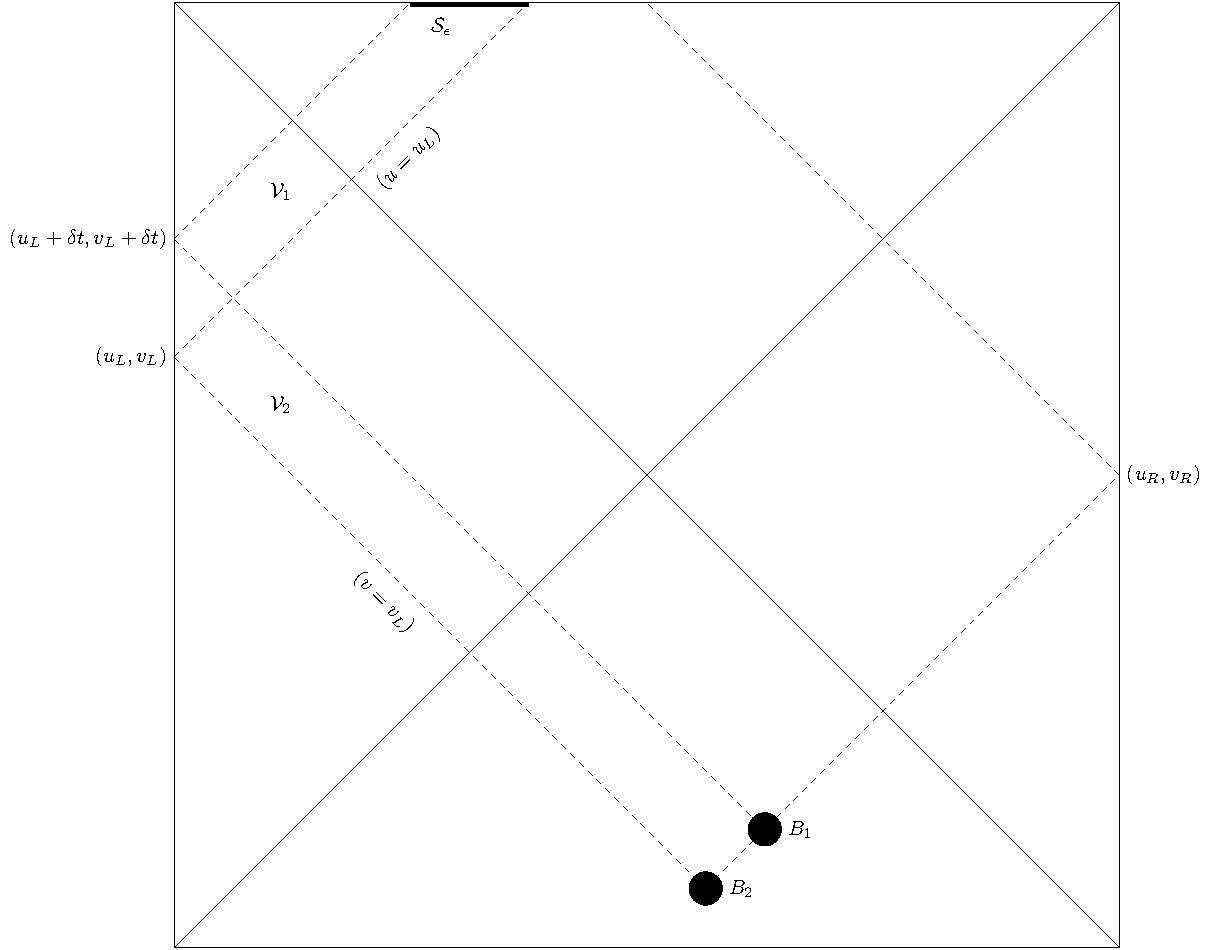
\includegraphics[scale=0.5]{WDW.pdf}    
    
    \end{center}
    \caption{Two WDW patches separated by $\delta t$.  Although the boundary of each patch is really at some large but finite $r_b$, the choice of $r_b$ drops out in the differences we consider and we do not indicate it explicitly in this graphic.}
    \label{fig:WDW}
\end{figure}

\end{frame}


%\section{The Gravity Dual of NCSYM}

\begin{frame}
\frametitle{Non-Commutative SYM}

\begin{itemize}

\item We would like to test complexity = action in a new context. However, computing the complexity of a state in a strongly couped field theory is not something we know how to do. Instead, we will rely on our intuition about the qualitative behavior of complexity in some novel situation.

\item A good candidate is SYM living on a non-commutative geometry, i.e., a geometry where two of the spatial directions don't commute.

\item A gravity dual to such a theory was derived in the late 90's by a number of authors \cite{Hashimoto:1999ut, Maldacena:1999mh}.

\item Generalizations of this system to other numbers of dimensions have also been considered in, e.g., \cite{Alishahiha:1999ci, Berman:2000jw}.

\item These solutions are obtained by considering a stack of Dp-branes in type II string theory and exciting a compenent of the NS-NS 2-form B-field along two of the worldsheet directions.

\item Additional non-commutativities can be introduced by turning on additional complenets of the B-field.

\end{itemize}

\end{frame}

\begin{frame}
\frametitle{The gravity dual to NCSYM}

The gravity dual to NCSYM is obtained in a manner similar to the standard commutative story.

\begin{itemize}

\item Consider a stack of D3-branes

\item we turn on a 2-form B parallel to the two spatial dimensions of the branes

\item This can be achieved by applying a combination of T-dualities and Gauge transformations

\item The B-field has the effect of introducing non-commutativity in the worldbrane theory

\item The near horizon geometry is a IIB SUGRA solution.

\item This procedure can be generalized to Dp-branes, with p = 2, 4, or 5.

\end{itemize}

\end{frame}

%\section{Results}

\begin{frame}
\frametitle{D3-brane results: Finite time behavior}

Similar behaviour to (cite paper by Rob, Shira, etc.), (of course as $a\rightarrow 0$ must reproduce planar black hole)

\begin{itemize}

\item Logarithmic divergence at critical time (smooth out with thermal average?)

\item Reaches true global maximum in order one time (in thermal units)

\item approaches asymptotic value from above

\item This behavior persists for all values of the Moyal scale ...

\item ... but as the Moyal scale becomes very large, the true maximum shrinks, and the asymptotic value increases, so that the gap between them decreases

\end{itemize}

This behaviour calls into question the normalization to complexity = action as set by (cite Brown et al.), though the logic that to that normalization would seem already to be contradicted by (cite Cotrell 'complexity is simple')

\end{frame}

\begin{frame}
\frametitle{D3-brane results: Late time limit}

We see a 25\% enhancement for large Moyal scale!

\begin{figure}[htbp]
    \begin{center}
        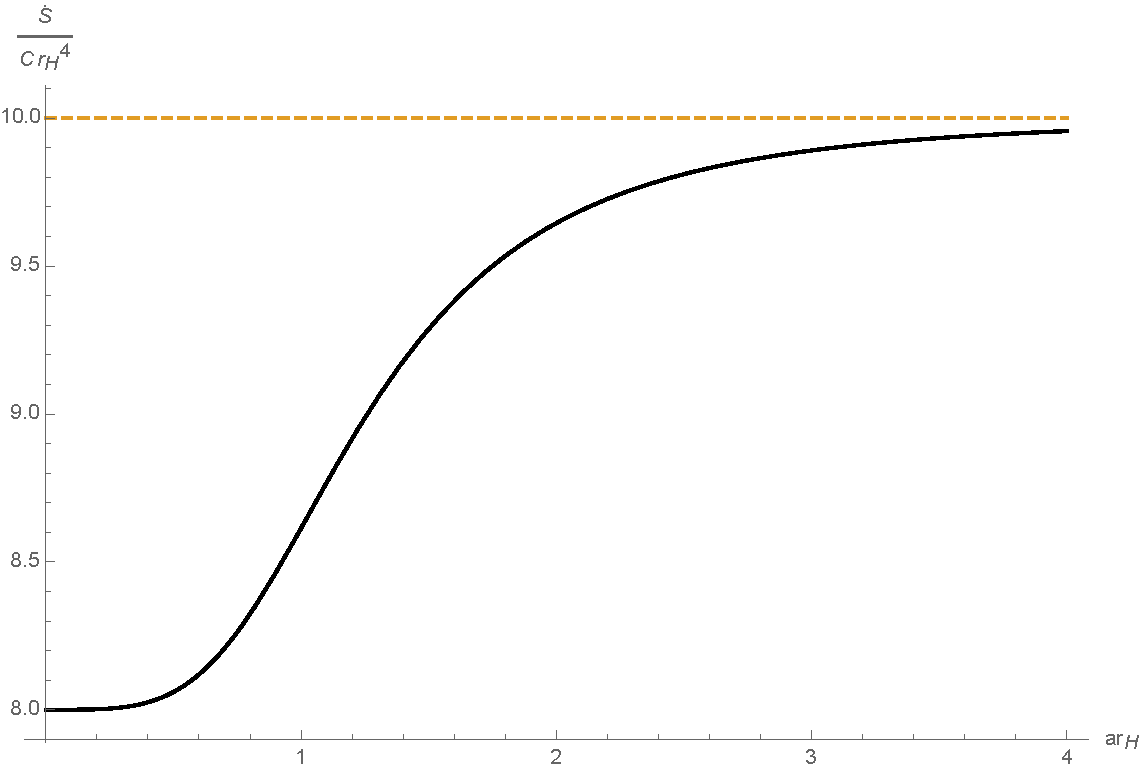
\includegraphics[scale=0.3]{LateTime}
    \end{center}
    \caption{Late time action growth rate normalized by $C=\frac{\alpha^4 \Omega_5 V_3}{\hat{g}_s^2}$ and extra $r_H$ dependence, versus $a r_H$, which is the Moyal scale measured in units of thermal length.} 
    \label{fig:LateTime}
\end{figure}

At first this seems a bit mysterious, but perhaps we should have expected it.

\end{frame}

\begin{frame}
\frametitle{Non-Commutativity and Complexity: A heuristic argument}

\begin{figure}
    \begin{center}
        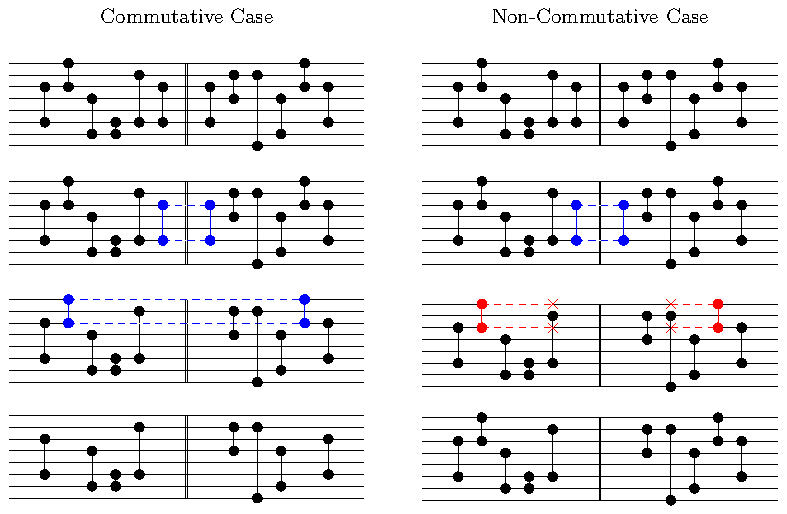
\includegraphics[scale=0.6]{cartoon}
    \end{center}
   \caption{Consider an optimal circuit that evolves our state by a small time $\delta t$. As we compose this circuit many times, we expect some cancelations between gates in adjacent copies of the ciruit. Non-commutativity acts as an impediment to such cancelation by making fewer gates commute (due to non-locality), and so the final ciruit after cancelation is more complex.} \label{fig:cartoon1}
\end{figure}

\end{frame}

\begin{frame}
\frametitle{Results for other values of $p$}

\begin{table}
    \centering
    \begin{tabular}{l | c  c  c }
        $p$ & $m=0$ & $m=1$ & $m=2$ \\
        \hline
        2 & 12 & 12 & - \\
        3 & 8 & 10 & - \\
        4 & 5 & 5 & 8 \\
        5 & 4 & 5 & 6 \\
    \end{tabular}
\end{table}

\end{frame}

\begin{frame}
\frametitle{Conclusions}

\begin{itemize}

\item For $p=3,5$ we do see an increase, as expected.

\item Though we did not see an increase for $p=2$ or for $p=4$ with a single non-trivial commutator, we did not see a decrease either.

\item Overall, the results are consistent with the heuristic argument above.

\item This result is in tension with the idea that commutative black holes are he fastest possible computers

\item In future work we plan to repeat our calculations for complexity = volume.

\end{itemize}

\end{frame}

\begin{frame}
\frametitle{References}

\bibliographystyle{JHEP} %JHEP.bst
\footnotesize\bibliography{NCG} %NCG.bib

\end{frame}

\section{Backup Slides}

\begin{frame}
\frametitle{Holographic Complexity}

\begin{itemize}

\item Consider a two sided black hole in asymptotically AdS space.

\item A holographic puzzle: what could be dual to the geometry behind the horizon?

	\begin{itemize}
	
	\item AdS/CFT $\Rightarrow$ a two sided black hole is dual to the thermofield double (TFD) state.
	
	\item The volume of the wormhole keeps growing long after the thermalization time	.
	
	\item This would seem to indicate that most observables we consider for a thermal state will fail.
	
	\item By contrast, the circuit complexity of a TFD state continues to grow long past the thermalization time
	
	\end{itemize}
	
\item (Possible) resolution: the behind the horizon geometry encodes the circuit complexity of the quantum state. 

\end{itemize}

\end{frame}

\begin{frame}
\frametitle{Quantum Circuit Complexity}

What is 'circuit complexity'?

\begin{itemize}

\item Consider a Hilbert space $\mathcal{H}$, e.g., the Hilbert space for $N$ quantum bits.

\item A universal gate set $\{g_i\}$ for $\mathcal{H}$ is a set of unitary operators on the Hilbert space such that any unitary $U$ acting on $\mathcal{H}$ can be approximated by some product $\displaystyle\prod_{i} g_{\alpha_i}$ to within a small tolerance $\epsilon$. 

\item Such a product of gates is referred to as a quantum circuit.

\item The quantum circuit complexity of a unitary $U$ is then the minimum number of gates needed to approximate $U$ to within the tolerance.

\item In the example of qubits, one typically considers gates that act on a single qubit or pairs of qubits at a time.

\item Given some reference state $\ket{\psi_R}$, one may define the complexity of a state $\ket{\psi}$ as the minimum of complexity $C(U)$ over all unitaries $U$ such that $\ket{\psi} = U\ket{\psi_R}$.

\end{itemize}

\end{frame}

\end{document}